\documentclass{beamer} 
\usepackage{amsmath,amsthm}
\usepackage{graphicx,microtype,parskip}
\usepackage{caption,subcaption,multirow}
\usepackage{attrib}

\frenchspacing

\usetheme{default}
\usecolortheme{whale}

\setbeamertemplate{navigation symbols}{}

\setbeamercolor{title}{fg=blue,bg=white}

\setbeamercolor{block title}{fg=white,bg=gray}
\setbeamercolor{block body}{fg=black,bg=lightgray}

\setbeamercolor{block title alerted}{fg=white,bg=darkgray}
\setbeamercolor{block body alerted}{fg=black,bg=lightgray}


\title{Taxon occurrence as a function of both biological traits and environmental context}
\subtitle{the changing North American species pool}
\author{Peter D Smits}
\institute{Committee on Evolutionary Biology, University of Chicago}
\titlegraphic{
  
\includegraphics[width=2.75cm,height=2.75cm,keepaspectratio=true]{figure/paleodb}
  \hspace*{0.35\paperwidth}
  
\includegraphics[width=2cm,height=2cm,keepaspectratio=true]{figure/chicago}
}
\date{}

\begin{document}

\begin{frame}
  \maketitle
\end{frame}


\begin{frame}
  \begin{alertblock}{Question}
    When are certain ecologies/ecotypes enriched or depleted?
  \end{alertblock}
\end{frame}


\begin{frame}
  \frametitle{Cenozoic mammals of North America}
  \begin{center}
    \includegraphics[height=0.8\textheight,width=\textwidth,keepaspectratio=true]{figure/Miocene}
  \end{center}

  \attrib{\footnotesize{Matternes, 1964}}
\end{frame}


\begin{frame}
  \frametitle{Differences in extinction risk}

  \begin{center}
    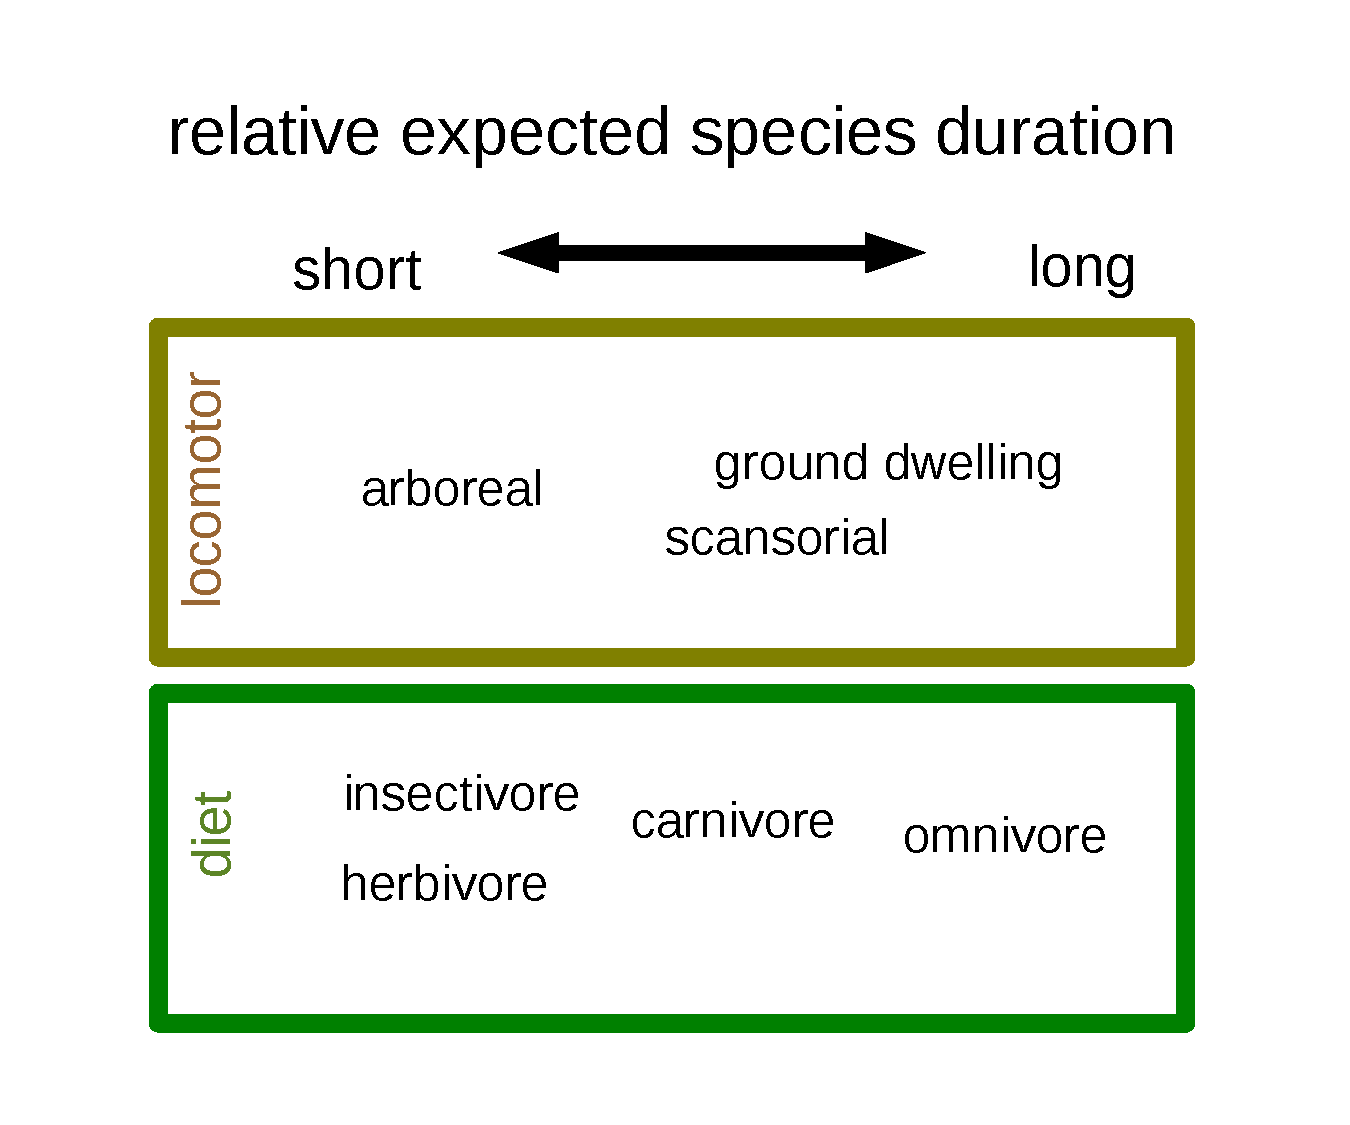
\includegraphics[height=0.8\textheight,width=\textwidth,keepaspectratio=true]{figure/smits_2015_results}
  \end{center}

  \attrib{\footnotesize{Smits, 2015, \em{PNAS}}}
\end{frame}


\begin{frame}
  \frametitle{Species pool concept}

  \begin{center}
    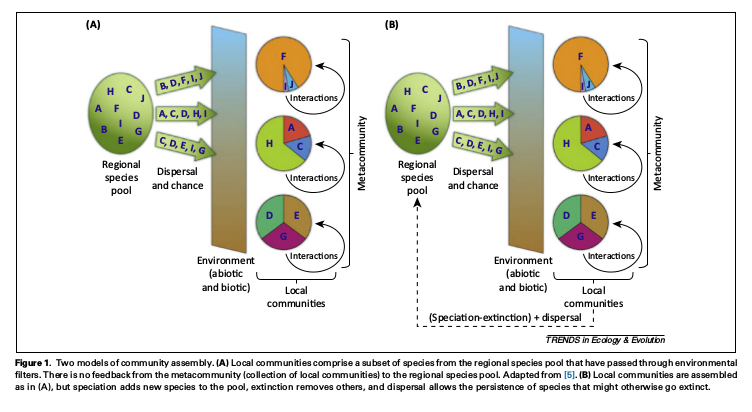
\includegraphics[height=0.8\textheight,width=\textwidth,keepaspectratio=true]{figure/schemske_pool}
  \end{center}

  \attrib{\footnotesize{Mittelbach and Schemske, 2015, \em{TREE}}}
\end{frame}


\begin{frame}
  \frametitle{Eco-cube and ecotypes}

  \begin{center}
    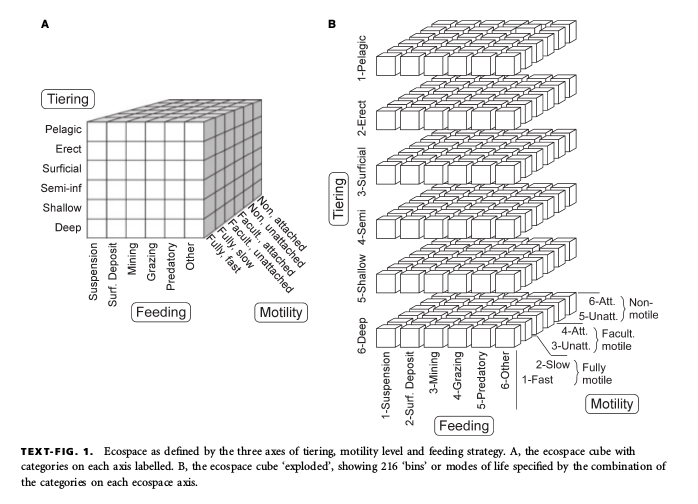
\includegraphics[height=0.8\textheight,width=\textwidth,keepaspectratio=true]{figure/ecocube}
  \end{center}

  \attrib{\footnotesize{Bambach \em{et al.}, 2007, \em{Palaeontology}}}
\end{frame}

\begin{frame}
  \frametitle{The fourth-corner problem}

  \begin{center}
    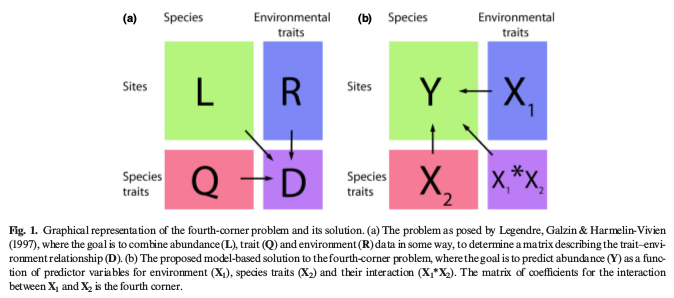
\includegraphics[height=0.8\textheight,width=\textwidth,keepaspectratio=true]{figure/warton_fourth_corner}
  \end{center}

  \attrib{\footnotesize{Brown \em{et al.}, 2014, \em{Methods Ecol. Evol.}}}
\end{frame}

\begin{frame}
  \frametitle{A worked example of a fourth-corner model}

  \begin{columns}
    \begin{column}{0.4\textwidth}
      \begin{itemize}
        \item Pollock \textit{et al.} 2012 Ecography
        \item eucalypts in Australia
        \item species traits: plant height, leaf area, seed mass
        \item environmental traits: rockiness, valley flatness, 
          precipitation, temp seasonality, solar radiation, soil sand, soil loam
      \end{itemize}
    \end{column}
    \begin{column}{0.6\textwidth}
      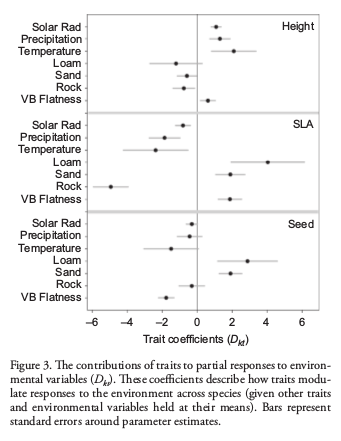
\includegraphics[height=0.8\textheight,width=\textwidth,keepaspectratio=true]{figure/pollock_trees}
    \end{column}
  \end{columns}
\end{frame}

\begin{frame}
  \frametitle{Paleo-fourth corner model}

  \begin{center}
    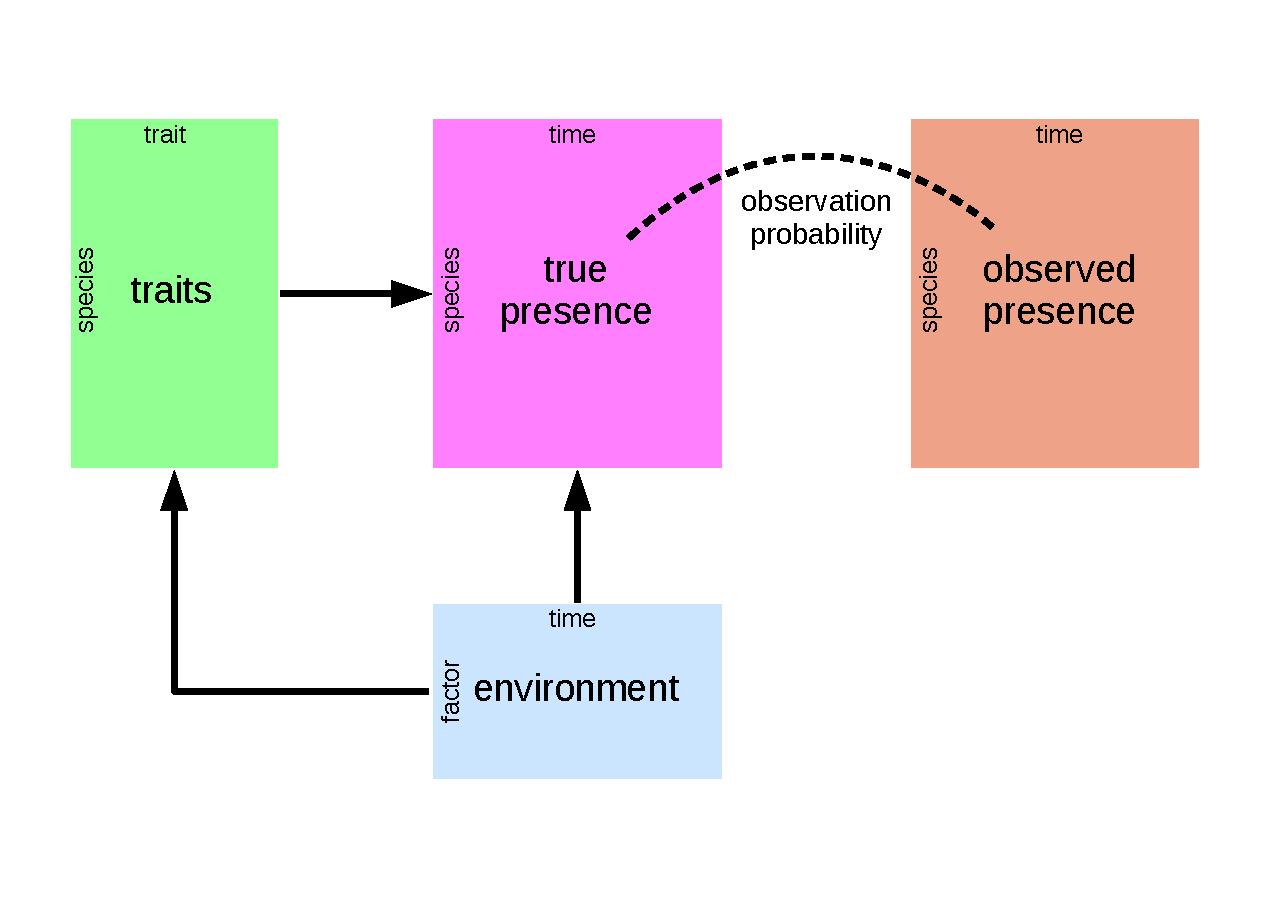
\includegraphics[height=0.8\textheight,width=\textwidth,keepaspectratio=true]{figure/paleo_fourth_corner}
  \end{center}
\end{frame}


\begin{frame}
  \frametitle{Covariates of interest}
  \begin{columns}
    \begin{column}{0.5\textwidth}
      individual-level \\(species i at time unit t)
      \begin{itemize}
        \item log-odds of occurrence probability at time t
        \item effect of locomotor type
          \begin{itemize}
            \item arboreal, digitigrade, plantigrade, unguligrade, fossorial, scansorial
          \end{itemize}
        \item effect of dietary type
          \begin{itemize}
            \item carnivore, herbivore, insectivore, omnivore
          \end{itemize}
        \item effect body size \\(rescaled log body mass)
      \end{itemize}
    \end{column}
    \begin{column}{0.5\textwidth}
      group-level (2 My time unit t)
      \begin{itemize}
        \item overall mean of log-odds of occurrence probability
        \item temperature record based on Mg/Ca estimates
          \begin{itemize}
            \item mean and interquartile range of rescaled value
          \end{itemize}
        \item plant community phase following Graham 2011
      \end{itemize}
    \end{column}
  \end{columns}
\end{frame}


\begin{frame}
  \frametitle{Model of taxon occurrence}
  \begin{itemize}
    \item response is p/a of genus in NA at time \(t\)
      \begin{itemize}
        \item Bernoulli variable 
        \item probability is (observation prob) times (``true'' presence)
      \end{itemize}
    \item observation probability is effect of sampling/fossil record
      \begin{itemize}
        \item basic model does not model sampling
      \end{itemize}
    \item the latent discrete ``true'' presence modeled as a \\multi-level logistic regression
      \begin{itemize}
        \item individual- and group-level
      \end{itemize}
  \end{itemize}
\end{frame}


\begin{frame}
  \frametitle{Paleo-fourth corner model}

  \begin{center}
    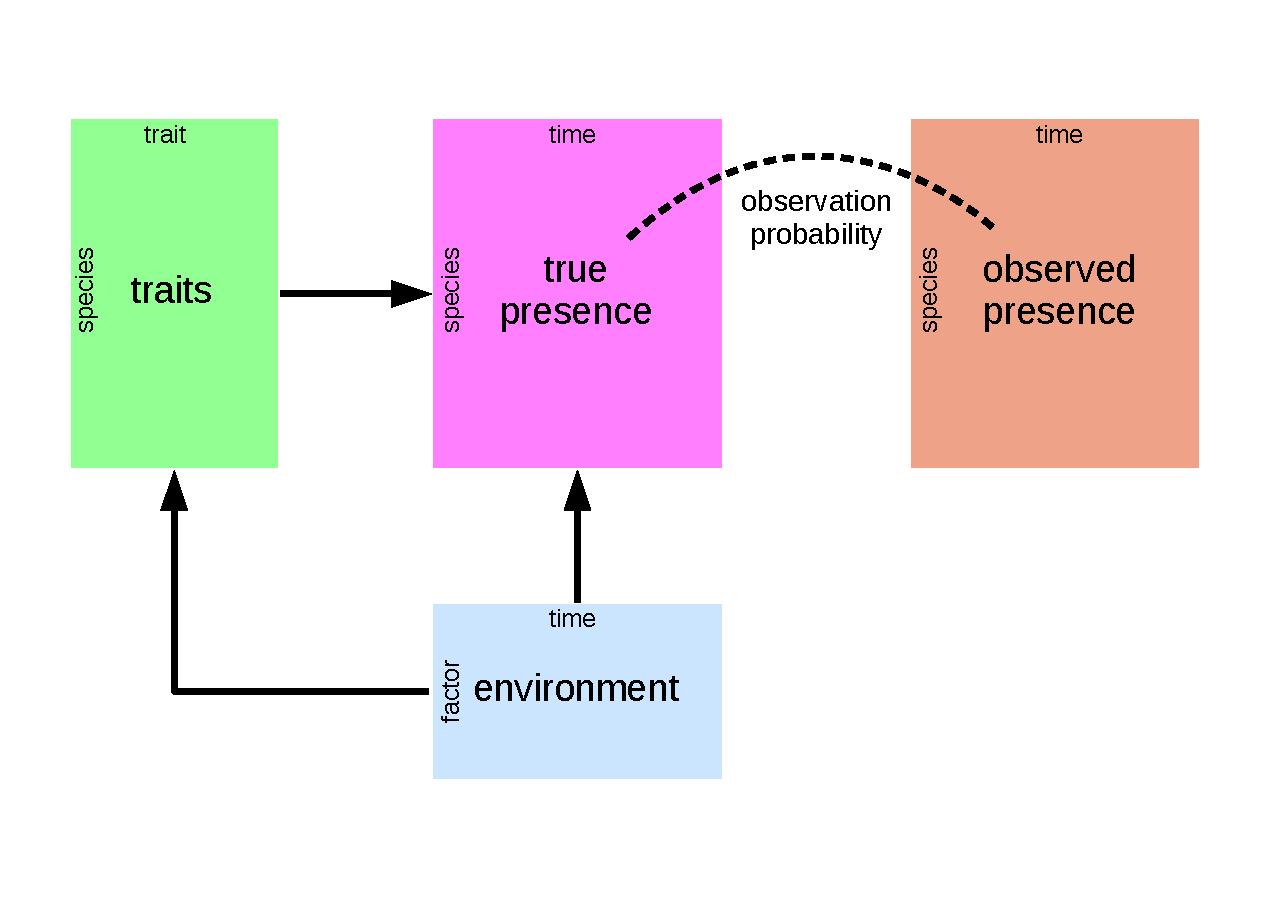
\includegraphics[height=0.8\textheight,width=\textwidth,keepaspectratio=true]{figure/paleo_fourth_corner}
  \end{center}
\end{frame}


\begin{frame}
  \frametitle{Model and sampling statement definition}
  \footnotesize{
    \begin{align*}
      y_{i,t} &\sim \text{Bernoulli}(\rho_{t} z_{i,t}) \\
      \text{logit}(\rho_{t}) &\sim \mathcal{N}(\rho^{'}, \sigma_{\rho}) \\
      z_{i,t} &\sim \text{Bernoulli}(\theta_{i, t}) \\
      \text{logit}(\theta_{i, t}) &= z_{i,t-1} (X_{i} \beta_{t\_}) + (\prod_{k = 1}^{t-1} 1 - z_{i,k}) (X_{i} \beta_{t\_}) \\
      \beta_{t} &\sim \text{MVN}(\mu, \Sigma) \\
    \end{align*}
  }
  \scriptsize{Note: Product term ensures taxon-loss is permanent. Implementation in Stan marginalizes over all possible (range-through) values of \(z\) instead of estimating the discrete parameters. I also use a noncentered parameterization of the hierarchical effects for better posterior sampling behavior. This presentation excludes final (hyper)priors.}
\end{frame}


\begin{frame}
  \frametitle{Parameter estimation and inference}

  \begin{columns}
    \begin{column}{0.45\textwidth}
      \begin{itemize}
        \item full HMC/MCMC slow
        \item Automatic Differentiation Variational Inference (ADVI) 
          \begin{itemize}
            \item approximate Bayesian inference
            \item assumes posterior is Gaussian, no correlation between parameters
            \item true Bayesian posterior
          \end{itemize}
      \end{itemize}
    \end{column}
    \begin{column}{0.55\textwidth}
      
\includegraphics[height=0.9\textheight,width=\textwidth,keepaspectratio=true]{figure/stan_logo}
    \end{column}
  \end{columns}
\end{frame}


\begin{frame}
  \frametitle{Posterior predictive performance}

  \begin{center}
    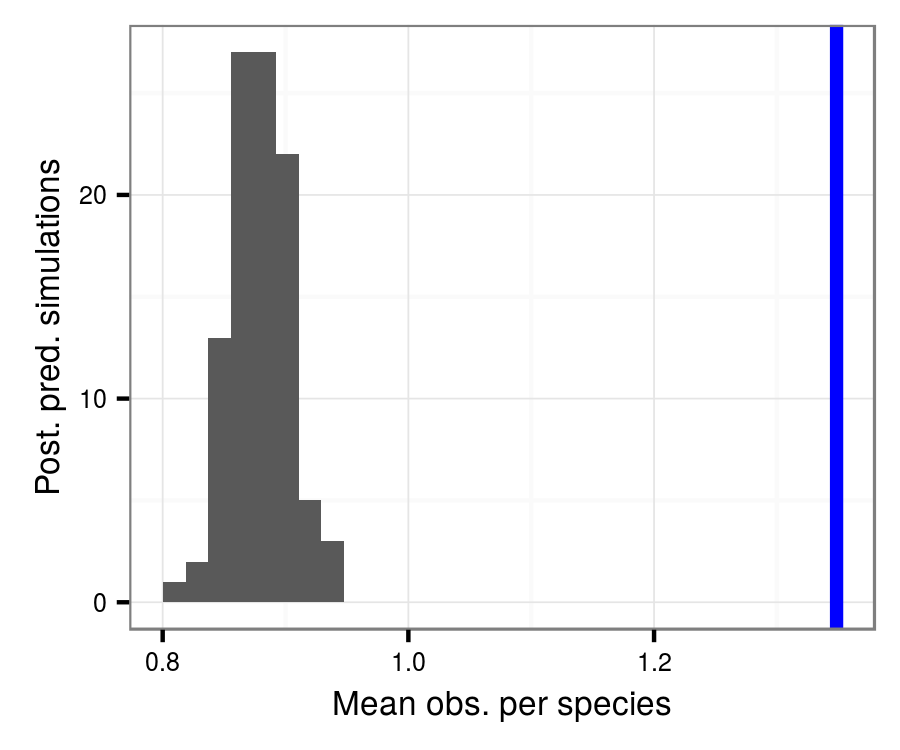
\includegraphics[height=\textheight,width=\textwidth,keepaspectratio=true]{figure/pred_occ}
  \end{center}
\end{frame}


\begin{frame}
  \frametitle{Effect of mass on log-odds of occurrence}

  \begin{columns}
    \begin{column}{0.5\textwidth}
      Basic model
      \vspace*{0.05\textheight}

      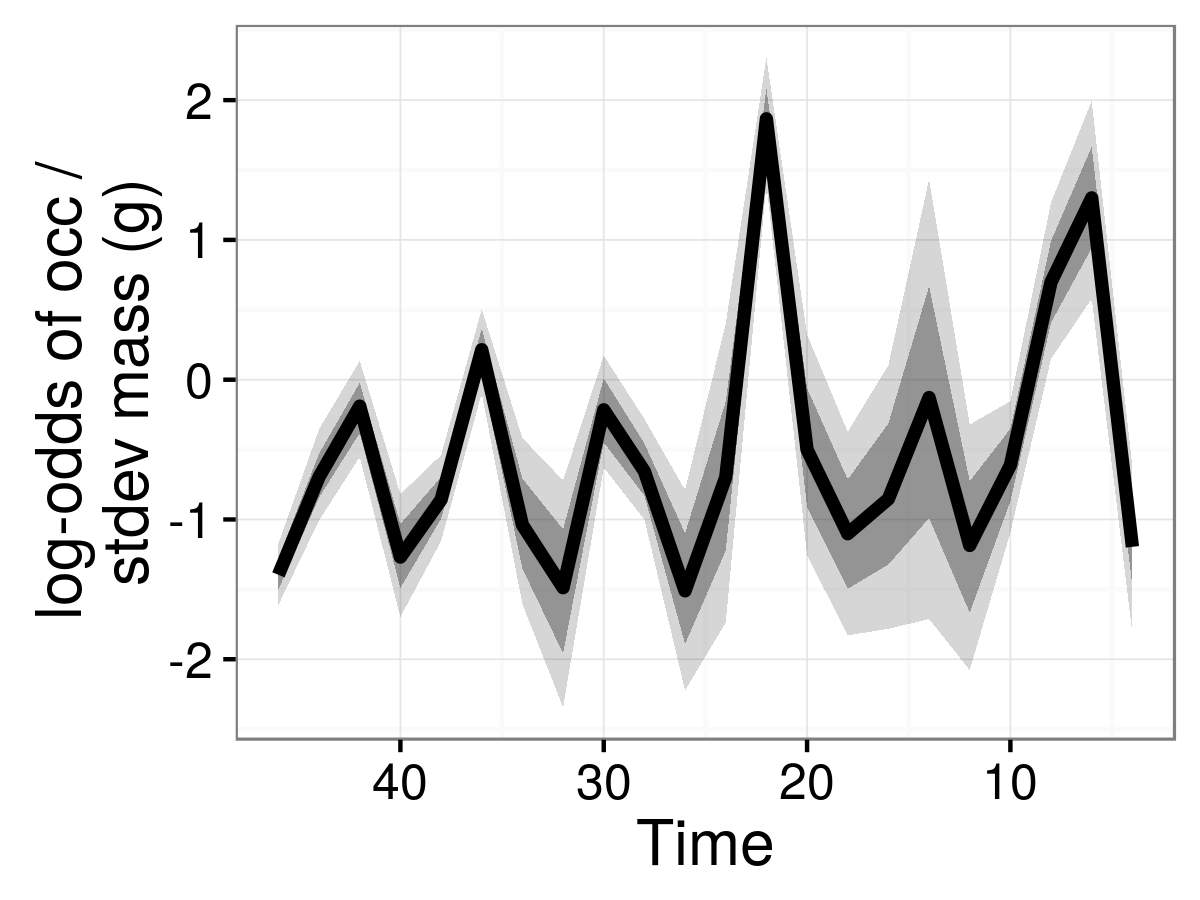
\includegraphics[height=\textheight,width=\textwidth,keepaspectratio=true]{figure/mass_eff_basic}
    \end{column}
    \begin{column}{0.5\textwidth}
      Full model
      \vspace*{0.05\textheight}

      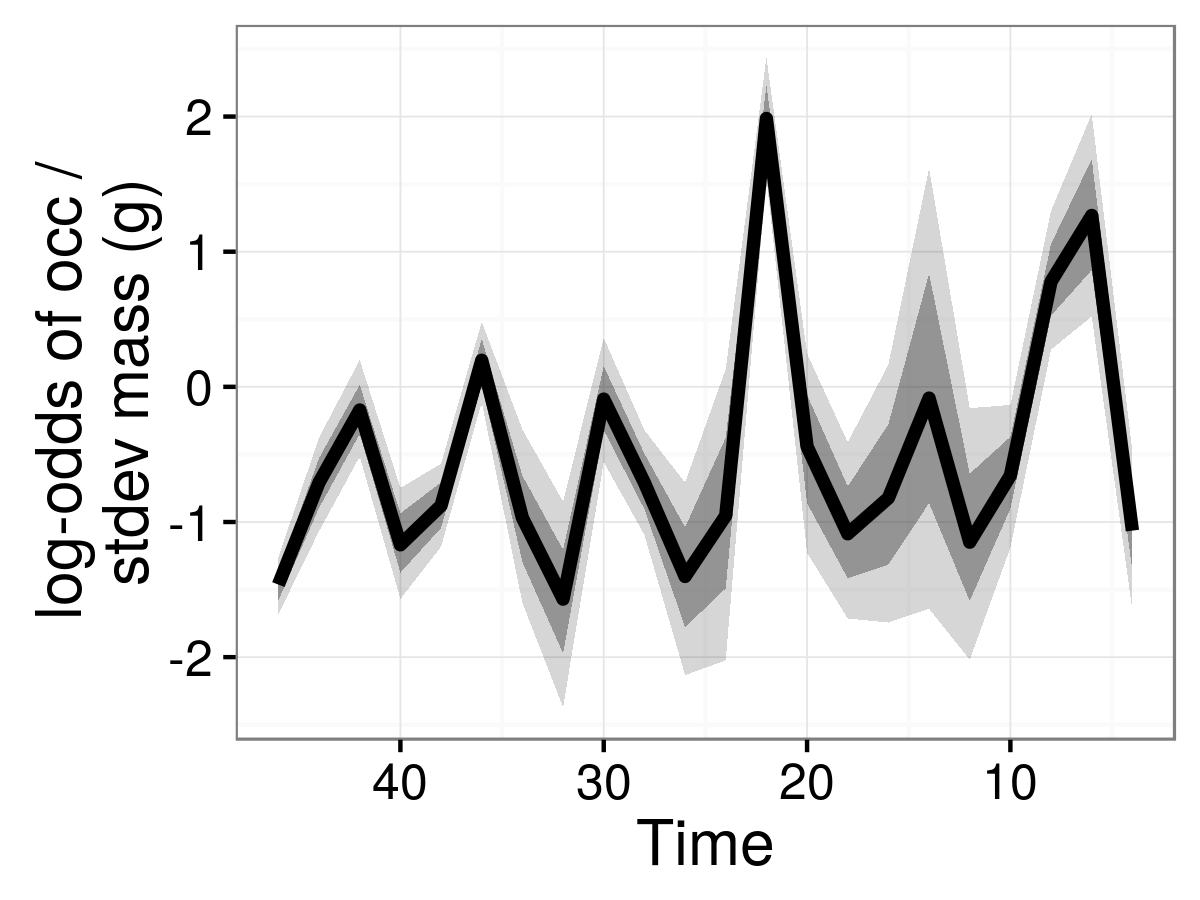
\includegraphics[height=\textheight,width=\textwidth,keepaspectratio=true]{figure/mass_eff_full}
    \end{column}
  \end{columns}
\end{frame}


\begin{frame}
  \frametitle{Probability occurrence is of ecotype (basic model)}

  \begin{center}
    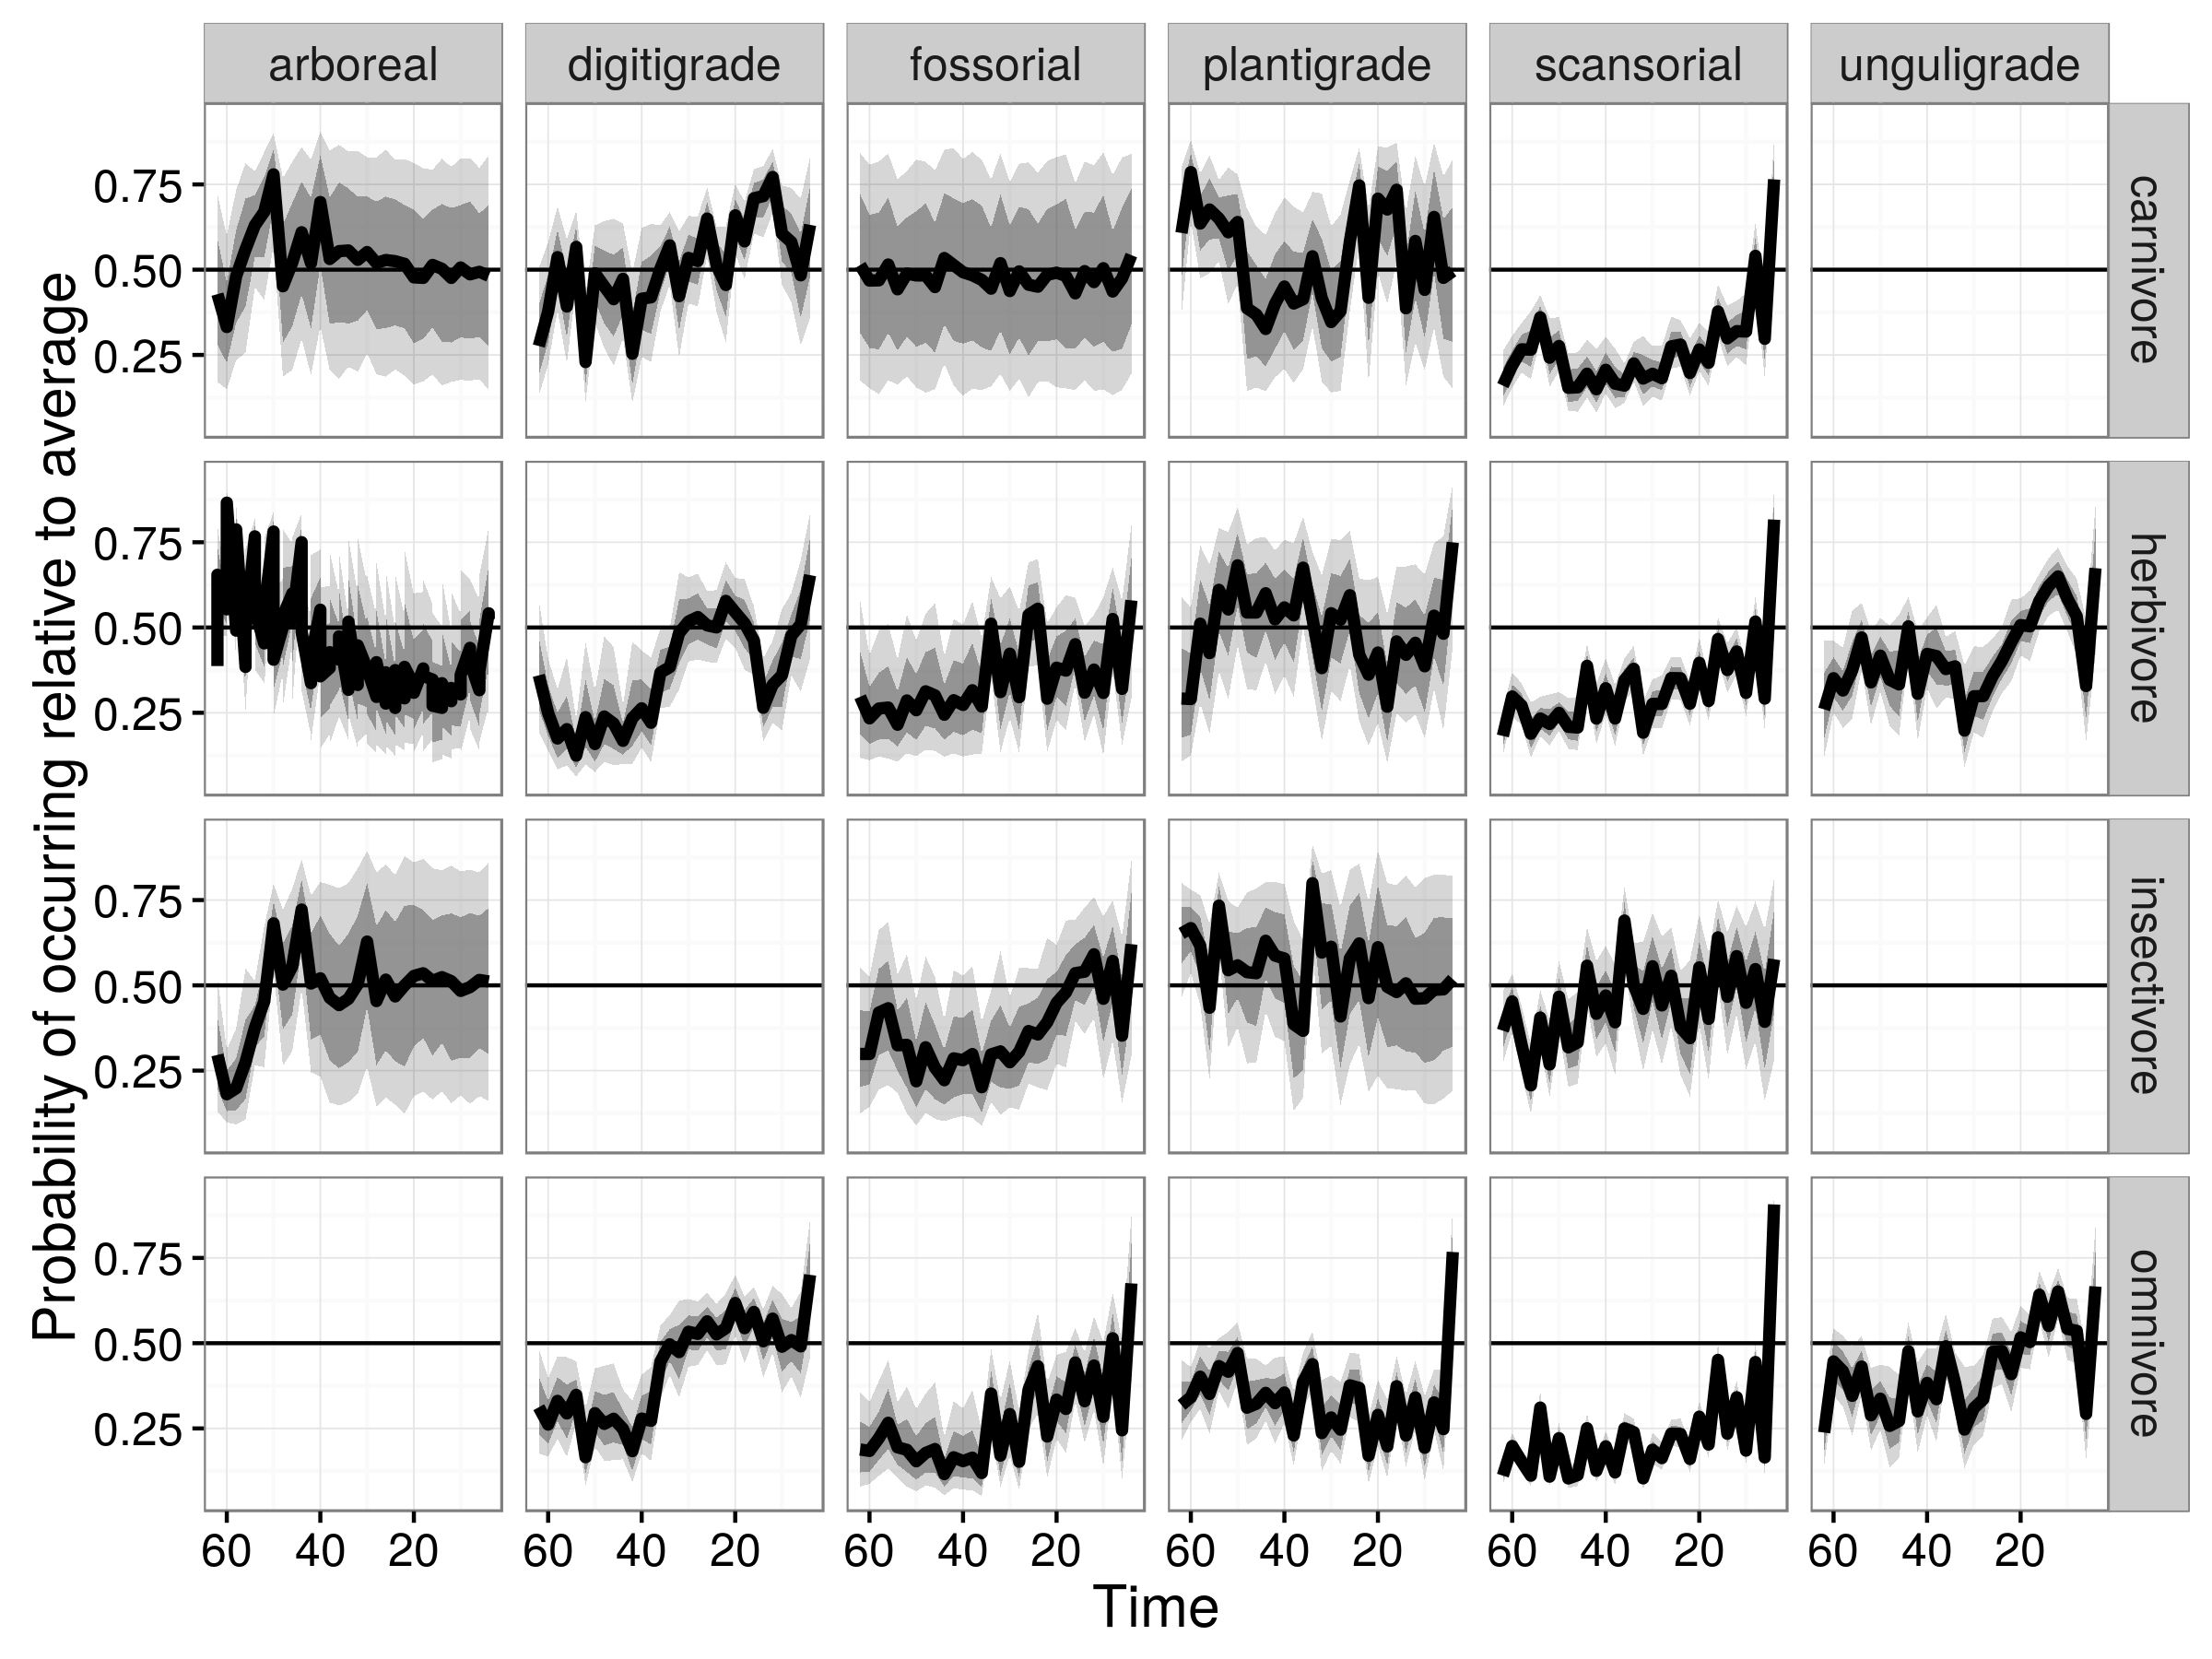
\includegraphics[height=0.8\textheight,width=\textwidth,keepaspectratio=true]{figure/cept_occur_prob_basic}
  \end{center}
\end{frame}


\begin{frame}
  \frametitle{Probability occurrence is of ecotype (full model)}

  \begin{center}
    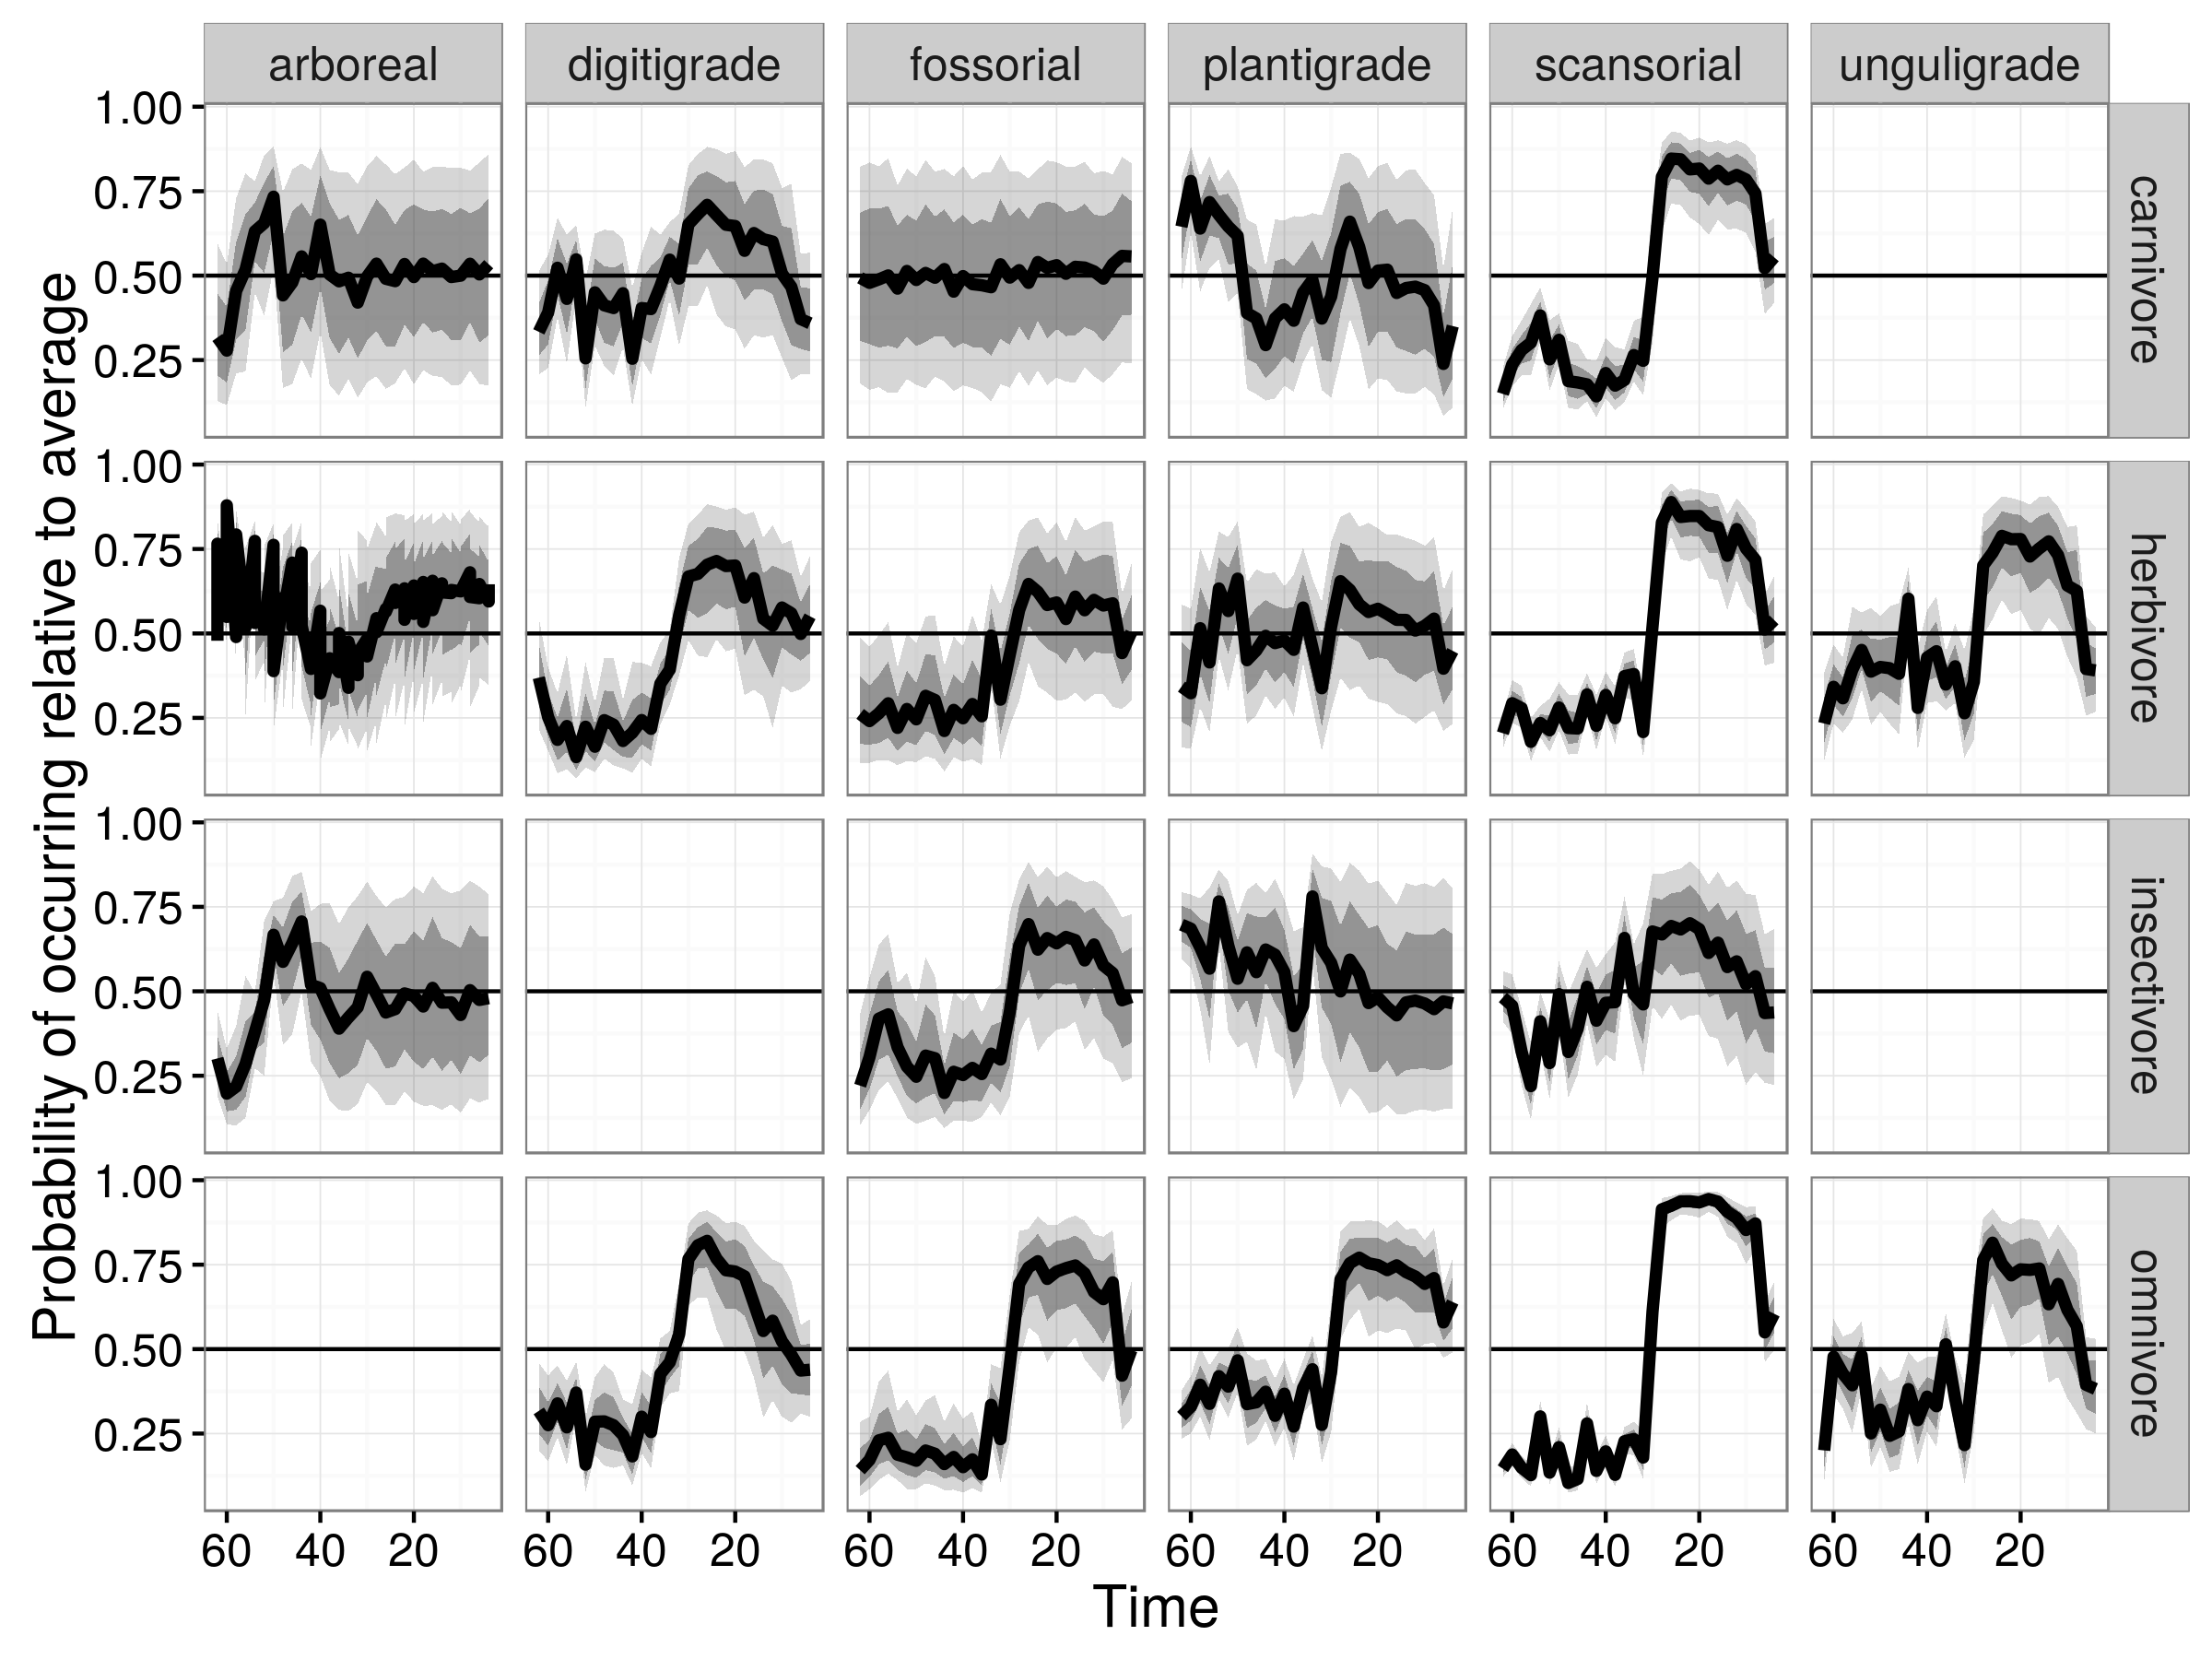
\includegraphics[height=0.8\textheight,width=\textwidth,keepaspectratio=true]{figure/cept_occur_prob_full}
  \end{center}
\end{frame}


\begin{frame}
  \frametitle{Group-level effects (plant phase, climate)}

  \begin{center}
    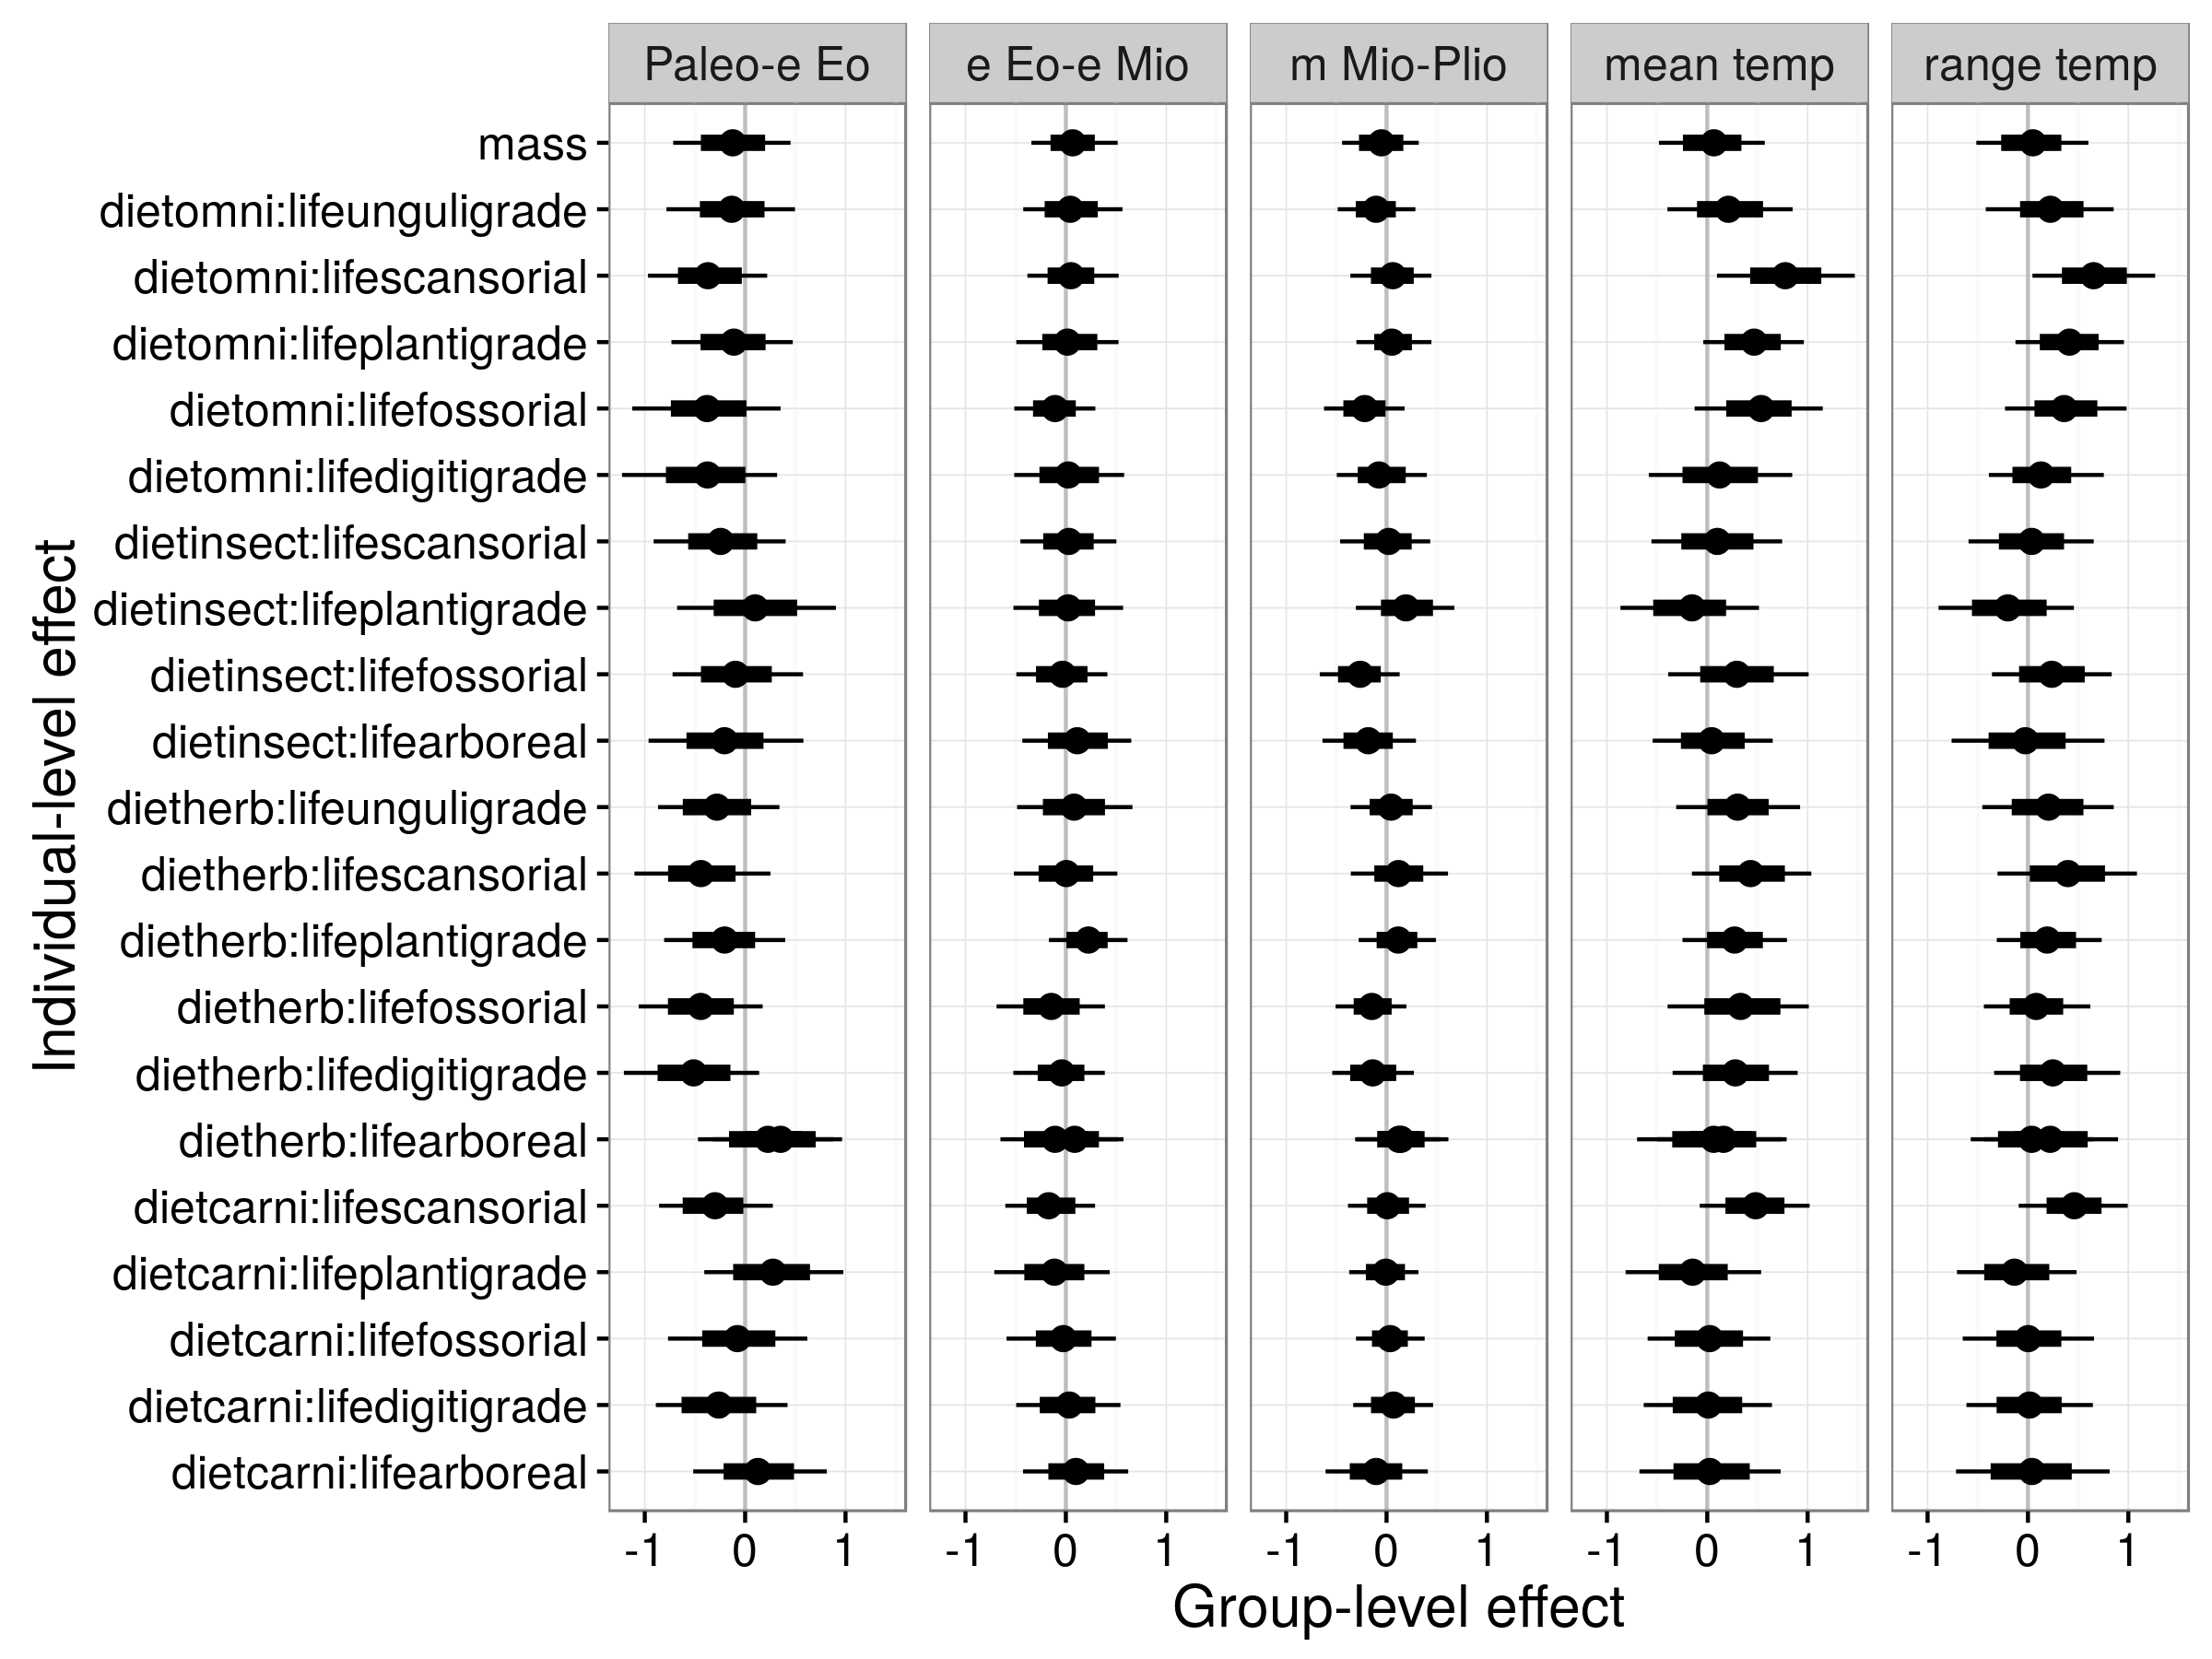
\includegraphics[height=0.8\textheight,width=\textwidth,keepaspectratio=true]{figure/gamma_est_full}
  \end{center}
\end{frame}


\begin{frame}
  \begin{block}{Concerns and conclusions}
    \begin{itemize}
      \item basic and full models have similar results until Neogene
      \item posterior predictive simulations disimilar to observed; poor model adequacy
        \begin{itemize}
          \item previous work has \emph{never} evaluated model adequacy
          \item second-order Markov process?
          \item full posterior inference?
        \end{itemize}
      \item decreasing ability to discern arboreal taxa over time (absence/increased rarity)
      \item increase in scansorial taxa over time
      \item increase in herbivorous taxa over time
      \item plant phase has small, idiosyncratic effects
    \end{itemize}
  \end{block}
\end{frame}


\begin{frame}
  \frametitle{Acknowledgements}
  \begin{columns}
    \begin{column}{0.5\textwidth}
      \begin{itemize}
        \item Advising
          \begin{itemize}
            \item Kenneth D. Angielczyk, Michael J. Foote, \\P. David Polly, \\Richard H. Ree, \\Graham Slater
          \end{itemize}
        \item Angielczyk Lab
          \begin{itemize}
            \item {\small{David Grossnickle, \\Dallas Krentzel, \\Jackie Lungmus}}
          \end{itemize}
        \item Foote lab
          \begin{itemize}
            \item {\small{Marites Villarosa Garcia, \\Nadia Pierrehumbert}}
          \end{itemize}
      \end{itemize}
    \end{column}
    \begin{column}{0.5\textwidth}
      \begin{itemize}
        \item {\footnotesize{David Bapst, Ben Frable, \\Graeme Lloyd, Matt Pennell}}
        \item {\footnotesize{UChicago CEB}}
      \end{itemize}

      \vspace*{0.05\textheight}
      \begin{center}
        
\includegraphics[height=0.4\textheight,width=\textwidth,keepaspectratio=true]{figure/paleodb}
      \end{center}
    \end{column}
  \end{columns}
\end{frame}

\end{document}
